\documentclass[12pt]{report}%

\usepackage[utf8]{inputenc}
\usepackage[english]{babel}
\usepackage[T1]{fontenc}
\usepackage{beramono}
\usepackage{xcolor}
\usepackage{natbib}
\usepackage[Lenny]{fncychap}

%\setlength{\headheight}{15pt}
%\usepackage[llbracket]{stmaryrd}

\usepackage{titlesec}
\titleformat{\section}
{\Large\bfseries\rm}
	{\thesection}{1em}{}

\titleformat{\subsection}
{\large\bfseries\rm}
	{\thesubsection}{1em}{}

\usepackage{fancyhdr}
\pagestyle{fancy}

\fancyhf{}
\lhead{}
\rhead{\rightmark}
\cfoot{\thepage}

\usepackage{booktabs}
\usepackage{xspace}

\usepackage[linktocpage=true]{hyperref}
\hypersetup{
    colorlinks,
    %linkcolor={MidnightBlue},
    linkcolor={blue},
    %citecolor={MidnightBlue},
    citecolor={blue},
    %urlcolor={BrickRed}
}

\usepackage{listings}
\usepackage{tikz}

\usepackage{pgfplots}
\pgfplotsset{compat=newest}

% This allows `code` and @code@ to be used inside an lstlisting environment, highlighted with a color box.
% Blatantly stolen from: https://tex.stackexchange.com/a/49309
\makeatletter
\newenvironment{btHighlight}[1][]
{\begingroup\tikzset{bt@Highlight@par/.style={#1}}\begin{lrbox}{\@tempboxa}}
{\end{lrbox}\bt@HL@box[bt@Highlight@par]{\@tempboxa}\endgroup}

\newcommand\btHL[1][]{%
  \begin{btHighlight}[#1]\bgroup\aftergroup\bt@HL@endenv%
}
\def\bt@HL@endenv{%
  \end{btHighlight}%   
  \egroup
}
\newcommand{\bt@HL@box}[2][]{%
  \tikz[#1]{%
    \pgfpathrectangle{\pgfpoint{1pt}{0pt}}{\pgfpoint{\wd #2}{\ht #2}}%
    \pgfusepath{use as bounding box}%
    \node[anchor=base west, fill=orange!30,outer sep=0pt,inner xsep=1pt, inner ysep=0pt, rounded corners=3pt, minimum height=\ht\strutbox+1pt,#1]{\raisebox{1pt}{\strut}\strut\usebox{#2}};
  }%
}
\makeatother

\lstset{language=C++,
  basicstyle=\small\ttfamily,
  keywordstyle=\color{blue}\ttfamily,
  stringstyle=\color{red}\ttfamily,
  commentstyle=\color{magenta}\ttfamily,
  frame=l,
  prebreak=\raisebox{0ex}[0ex][0ex]{\ensuremath{\hookleftarrow}},
  breaklines=true,
  breakatwhitespace=true,
  tabsize=4,
  %escapeinside={@}{@},
  numbers=left,
  xleftmargin=.6cm,
  showstringspaces=false,
  captionpos=b,
  emph={malloc, realloc, calloc, free},
  emphstyle=\color{purple},
  escapeinside={(@}{@)},
  moredelim=**[is][\btHL]{`}{`},
  moredelim=**[is][{\btHL[fill=red!30,draw=yellow,dashed,thin]}]{@}{@},
  moredelim=**[is][{\btHL[fill=blue!20,draw=white,dashed,thin]}]{\$}{\$},
}

\lstdefinestyle{tiny}{
  basicstyle=\scriptsize\ttfamily
}

\newcommand{\todo}[1]{\textbf{\textcolor{red}{TODO: #1}}}

\title{Dangless: Safe Dangling Pointer Errors}
\author{Gábor Kozár}
\date{\today}

\usepackage{textcomp}
\begin{document}

\makeatletter
\begin{titlepage}
	\centering
	
\includegraphics[width=0.15\textwidth, trim={0 0.15cm 0 0}, clip]{img/vu.png} \hspace{1.3cm}
	
\includegraphics[width=0.15\textwidth, trim={0 0.74cm 0 0}, clip]{img/uva.eps}\par\vspace{1cm}
	{\scshape\huge Vrije Universiteit Amsterdam \par Universiteit van Amsterdam \par}

	\vspace{1.5cm}

	{\scshape\LARGE Master's thesis\par \par
		\vspace{0.2cm}
		\small \textit{Submitted in partial fulfillment of the requirements for\\ the joint degree of Master of Science in Computer Science.}\par}
	\vspace{1.5cm}

	{\Huge\bfseries \rm \textbf{\@title}\par}
	\vspace{1.5cm}

	{\Large\itshape\rm \noindent\textit{\@author}\\}
	\vspace{1mm}
	\textit{(VU ID: 2574038, UvA ID: 11158190)}
	\vfill

	\rm \noindent \textit{supervisors} \\ \vspace{0.15cm}
	%\begin{tabular}{r@{\hskip 0.4in}l}
	%	\rm \textbf{Vrije Universiteit Amsterdam} & \textbf{ING} \\
	%	dr.\ J.C.\ \textsc{Blanchette} & ir. R.W.\ \textsc{van Dalen} \\
	%	prof.\ dr.\ W.J.\ \textsc{Fokkink}
	%\end{tabular}
	\rm \textbf{Vrije Universiteit Amsterdam} \\
	prof.\ dr.\ H. \textsc{Bos} \\
	assistant prof.\ dr.\ C. \textsc{Giuffrida} \\
	dr.\ K. \textsc{Koning}
	\vfill
	
	{\large \@date\par}
\end{titlepage}
\makeatother

%\include{chapters/preface}

\tableofcontents
\listoffigures

\newpage

Abstract

Manual memory management required in programming languages like C and C++ has its advantages, but comes at a significant cost in complexity, frequently leading to bugs and security vulnerabilities. One such example is temporal memory errors, whereby an object is accessed after it has been deallocated, through a pointer (or C++ reference) that outlived it: a dangling pointer. Such bugs, even after decades of research and development both in tooling and programming languages, are still extremely common today.

We propose a new solution, called Dangless, which protects against temporal memory errors by ensuring that any memory accesses through dangling pointers are detected immediately and cause the application to be terminated. This is achieved by maintaining a unique virtual alias for each individual allocation, similarly to the shadow pages in previous work such as Electric Fence~\cite{electric-fence} and Oscar~\cite{oscar2017}. Dangless iterates on these existing techniques by significantly improving performance by running the process in a light-weight virtual environment, giving us direct access to the page tables and allowing us to remap virtual pages and modify page protection flags without having to pay the overhead of system calls.

We have evaluated performance on the SPEC2006 benchmarking suite and have found a geometric mean of 5.7\% runtime performance overhead and 8.2\% physical memory overhead. This makes Dangless one of the best-performing tools for preventing temporal memory errors, although its practical usefulness is reduced by not offering protection against a more widespread set of memory errors.

\chapter{Introduction}
\label{ch:intro}

\section{Memory errors}

Developing software is difficult. Developing software that is bug-free is all but impossible. Programming languages like C and C++ (the so-called ``low-level'' programming languages~\footnote{``low-level'' is traditionally used to indicate that the level of abstraction used by these  programming languages is relatively close to that of the hardware}) offer a great deal of control to the programmer, allowing them to write small and efficient computer programs. However, they also require the programmer to take a great deal of care with their development: the same level of control that allows extremely efficient software to be built also places a large burden on the developer, as making mistakes has steeper consequences than in high-level, safer programming languages (such as Java or C\#).

Typically, low-level programming languages require the programmers to manage memory manually, while higher-level languages generally include a garbage collector (GC) that frees the programmer from this burden. Managing memory manually means that objects whose lifetime is dynamic (not tied to a particular program scope) have to be \emph{allocated} as well as \emph{deallocated} (freed) explicitly.

In C, such memory allocation typically occurs using the \lstinline!malloc()! or \lstinline!calloc()! functions. These allocate a region inside the \emph{heap memory} of the application, reserving it for use, and returning a pointer (typically, an untyped \lstinline!void *!) to it. On the x86 and x86-64 architectures, which we will mainly concern ourselves with in this thesis, a pointer is just a linear memory address: a number representing the index of the first byte of the pointed region in the main memory. This makes pointer arithmetic, such as accessing \lstinline!numbers[4]! in a \lstinline!int *numbers! very easy and efficient to perform: just load \lstinline!sizeof(int)! bytes from the memory address \lstinline!(uintptr_t)numbers + 4 * sizeof(int)!. Conversely, after we are done with using a given memory region, we can and should deallocate it using the \lstinline!free()! function. This marks the memory region as no longer in use, and potentially reusable -- a characteristic that forms the basis of this thesis.

In C++, memory allocation typically happens using the \lstinline!new! or \lstinline!new[]! operators, and deallocation using the \lstinline!delete! or \lstinline!delete[]! operators. However, these behave exactly like \lstinline!malloc()! and \lstinline!free()! used in C in all ways that are important from a memory management point of view. I should note that in modern C++, the use of such memory management is discouraged and generally unnecessary since \emph{smart pointers} -- wrappers around pointers that automate the lifecycle management of the pointed memory region, conceptually similarly to a garbage collector -- were introduced. However, a lot of applications are still being developed and maintained that do not make use of such features.

Making mistakes with manual memory management is very easy. Allocating but not freeing a memory region even after it is no longer used is called a \emph{memory leak} and it increases the memory usage of the application, often in an unbounded manner, potentially until a crash occurs due to insufficient memory. Attempting to deallocate an object twice -- \emph{double free} -- causes the memory allocator to attempt to access accounting data stored typically alongside the user data in the since-freed region, often leading to seemingly nonsensical behaviour or a crash, given that the region may have been re-used. Accessing an offset that falls outside the memory region reserved for the object -- \emph{out-of-bounds access}, sometimes also called \emph{buffer overflow} or \emph{buffer underflow} -- can lead to reading unexpected data or overwriting an unrelated object, again often causing hard-to-understand bugs and crashes. One example for this would be attempting to write to \lstinline!numbers[5]! when only enough space to hold 5 elements was allocated, e.g.\ using \lstinline!int *numbers  = malloc(5 * sizeof(int))! (recall that in C and related languages, indexes start at 0, so the first item is located at index 0, the second at index 1, and so on). Finally, accessing a memory region that has been deallocated -- \emph{use after free} -- is similarly problematic. This generally occurs when a pointer is not cleaned up along with the object it referenced, leaving it dangling; often also called a \emph{dangling pointer}~\cite{dangling-ptr-smashing-webpdf}.

Besides the instability and general mayhem that such memory errors routinely cause, they can also leave the application vulnerable to attacks, for instance by enabling unchecked reads or writes to sensitive data, sometimes even allowing an attacker to hijack the control flow of the application, execute almost arbitrary instructions, and in essence take over the application.

It should be clear by now why modern, ``high-level'' programming languages restrict or completely prohibit the direct use of pointers, often by making it impossible and unnecessary to manage memory manually. In such languages, the programmer can perform allocations only by creating objects (preventing another class of bugs relating to the use of uninitialized memory), and leaving their deallocation to the runtime environment, commonly its component called the garbage collector (GC). The GC will periodically analyse the memory of the application, and upon finding objects that are no longer referenced, marks them for reclaiming, and eventually deallocating them automatically. This, of course, comes at a cost in performance, often one that is unpredictable as the GC is controlled by the runtime environment as opposed to the user code. (It is worth noting that this scheme does not protect against all possibilities of memory errors; for instance, leaks are still both possible and common.)

A notable exception is the Rust programming language, which, while does allow pointers, heavily restricts how they can be used, preventing any code that could potentially be unsafe. It does so using static (compile-time) checking using their so-called \emph{borrow checker}. However, realizing that in doing so it also disallows some valid uses of pointers, it also provides an escape hatch, allowing code sections to be marked as \emph{unsafe} and go unchecked. (For example, it is not possible to implement a linked list in safe Rust, and even the built-in \lstinline!vec! type is written using unsafe code.) Another programming language that follows a similar pattern is C\#: normally used as a high-level, managed language employing a GC, it also allows pointers to be used directly in code marked as unsafe~\footnote{Usage of raw pointers in an otherwise managed environment comes with caveats; for instance, the memory is often compacted after GC passes with the surviving objects moved next to each other to reduce fragmentation. Such relocation is not possible if there are raw pointers in play; therefore, programmers are required to mark the pointers they use as \emph{pinned} using the \lstinline!fixed()! construct.}.

Still, applications written in languages like C or (older) C++ with no safe alternatives to pointers have been written and are being maintained, and these applications remain affected by memory errors. Significant amount of research has been and continues to be conducted in this topic, as such applications are often high-value targets for attackers: operating system kernels, device drivers, web servers, anti-virus programs are commonly developed using these technologies.

This thesis is focused specifically on dangling pointer errors, a class of memory issues defending against which has traditionally been difficult and inefficient.

\section{Dangling pointers}

A pointer is said to be \emph{dangling} when it outlives the memory region it references. Dereferencing such a pointer will generally lead to unwanted, confusing behaviour.

In the very best-case scenario, the memory access fails, and the application is killed by the operating system kernel; for example on Unix systems by sending it a signal like \lstinline!SIGSEGV!, leading to the well-known ``Segmentation fault'' error and a groan from the programmer. This is useful (and often highly underrated by programmers), because it clearly indicates a bug, and the responsible memory address is readily available, greatly helping with debugging.

Unfortunately, in the majority of cases in practice, the memory access will not fail. The reason for this is that most modern architectures in widespread use (such as x86 and ARM) handle memory on the granularity of \emph{pages}, where a single page is usually 4096 bytes (4 kilobytes). From the point of view of the hardware and the kernel, a page is either in use or is not; pages are treated as a unit and are never split up. Of course, typical memory allocations tend to be significantly smaller than this, and it would be wasteful to dedicate an entire page of memory to just hold for instance 200 bytes of user data.

Therefore, all memory allocator implementations used in practice do split up pages, and will readily place two allocations on the same page, typically even directly next to each other (not counting any meta-data). After the deallocation of one of the objects, the page as a whole still remains in use, and so the hardware will not fault on subsequent accesses to it, regardless of the offset; see Figure~\ref{fig:mem_two_small_allocs}. Notably, even if a memory page holds no live objects, it is often still not returned to the system; the memory allocator retains it as an optimization, expecting more allocations in the future. (This is because the memory allocators being discussed run in user-space, so in order to gain access to memory pages to use, they have to perform a system call such as \lstinline|mmap()| or \lstinline|brk()|, which is costly.)

\begin{figure}
    \centering
    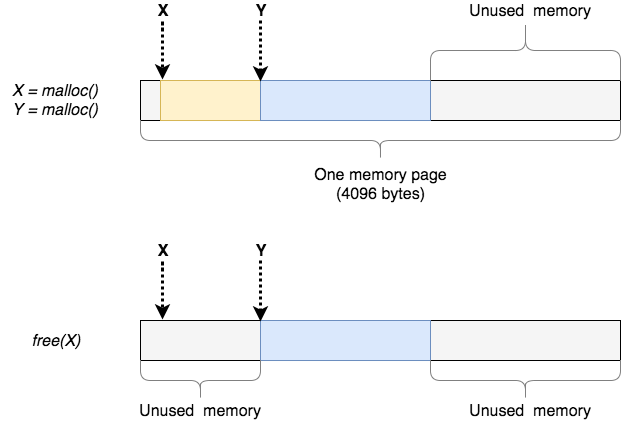
\includegraphics[width=\textwidth]{diagrams/dangling_pointer_basics.png}
    \caption{Memory layout of two small allocations. \emph{X} and \emph{Y} are pointers, referencing their corresponding memory regions. \emph{X} becomes dangling}
    \label{fig:mem_two_small_allocs}
\end{figure}

If a page is known to be unused by the hardware and kernel, then accessing it will trigger a page fault in the kernel, which will generally terminate the application, leading to the best-case scenario described earlier. This is a far more manageable problem than the alternative, because the error is clear, even if in practice it is often difficult to discover the underlying reason, given that time may have passed between the deallocation and attempted access, and so the code executing at the time of access may not have any relation to the code that was responsible for the deallocation. Furthermore, this scenario does not generally pose a security problem, as a crashed application is difficult to exploit. Therefore, I will generally ignore this scenario for the remainder of this thesis.

The effect of an unchecked access through a dangling pointer depends on whether or not the referenced memory region has been reused since the time of deallocation. If it has not, the data read often will still be valid, and execution may continue without anyone the wiser, masking the bug -- at least until a modification in the code or one of the libraries leads to a change in the memory allocation pattern. Otherwise, the dangling pointer will point inside another allocation, and the data read or overwritten will almost always be a source of unexpected behaviour: see Figure~\ref{fig:normal_malloc}.

\begin{figure}
	\centering
	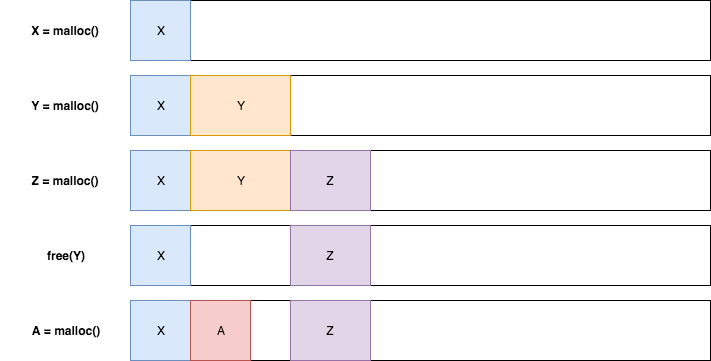
\includegraphics[width=\textwidth]{img/normal_malloc.png}
	\caption{(Simplified) Memory layout view when using traditional malloc(): memory is re-used}
	\label{fig:normal_malloc}
\end{figure}

One typical case is \emph{type confusion}: the value read or written will be treated as a different type than the value stored there. A string value can be for instance accessed as an integer, causing the characters that make up the string to be interpreted as bytes in an integer, essentially leading to the same behaviour as this code snippet:

\begin{lstlisting}
char *s = "foobar";
int i = *(int *)s;
\end{lstlisting}

This code compiles and runs successfully. What will be the value of \lstinline!i!? Of course, we are deep into undefined behaviour territory here, meaning that the programming language promises nothing. In practice, on x86-64 architectures where the \lstinline!int! C type is 4 bytes long (\lstinline!sizeof(int) == 4!), the result will typically be \texttt{1651470182}, or \texttt{0x626f6f66} in hexadecimal. This makes sense: the string \lstinline!"foobar"! (including the null terminator) is represented by the byte sequence \texttt{0x66 0x6f 0x6f 0x62 0x61 0x72 0x00}. Interpreting it as an \lstinline!int! means reading the first 4 bytes (\texttt{0x66 0x6f 0x6f 0x62}) and assembling it into a multi-byte integer according to the endianness of the processor. My laptop has an Intel CPU in it, which is little endian, meaning that the bytes of an integral type are stored as least significant byte first (this is \texttt{0x62}), followed by bytes of increasing significance; simply put, bytes are interpreted in ``reverse order''.

Of course, type confusion does not have to occur in order for invalid behaviour to occur. For instance, overwriting an Unix file descriptor with the number of characters in a text will typically result in an invalid file descriptor; or consider a buffer's length overwritten by the age of the user; or an integer representing the next free index in an array overwritten by the length of a file in bytes. Once memory corruption occurs, sanity flees.

\section{An example}

Let us look at a less trivial example. This is a simplistic codebase, written in C++ of an in-memory messaging system. Each \lstinline!User! has an inbox and outbox, \lstinline!Mailbox! objects, which wrap an \lstinline!std::vector<Message *>!. \lstinline!Message! objects are allocated on the heap, referenced by plain pointers, allowing the sender and recipient mailboxes to just both retain a pointer to the same message -- a memory optimization. Each message object keeps track of who has deleted it, and when both the sender and receiver have done so, the message can be safely deallocated.

\begin{lstlisting}
struct Message {
	const std::string mContent;

	$bool mHasSenderDeleted = false;$
	$bool mHasRecipientDeleted = false;$

	explicit Message(std::string content)
		:   mContent{std::move(content)}
	{}

	void OnDeleted() {
		@if (mHasSenderDeleted && mHasRecipientDeleted)@
			@delete this;@
	}
};

struct Mailbox {
	std::vector<Message*> mMessages;

	void AddMessage(Message* msg) {
		mMessages.push_back(msg);
	}

	void DeleteMessage(Message* msg) {
		mMessages.erase(std::find(mMessages.begin(), mMessages.end(), msg));
		msg->OnDeleted();
	}
};

struct User {
	Mailbox mInbox;
	Mailbox mOutbox;

	void SendMessage(User& recipient, std::string content) {
		Message* msg = new Message{std::move(content)};

		mOutbox.AddMessage(msg);
		recipient.mInbox.AddMessage(msg);
	}

	void DeleteReceivedMessage(Message* msg) {
		`msg->mHasRecipientDeleted = true;`
		mInbox.DeleteMessage(msg);
	}

	void DeleteSentMessage(Message* msg) {
		`msg->mHasSenderDeleted = true;`
		mOutbox.DeleteMessage(msg);
	}
};
\end{lstlisting}

The noteworthy lines have been highlighted. While this design is error-prone, as we will see, it does work correctly and does not -- in its current form -- represent a vulnerability.

However, code evolves over time as bugs are fixed and new features are added, often by a different developer than the original authors. Sometimes these programmers understand the codebase less, or have less experience with programming or the technologies used, and can easily make mistakes. Especially with a language like C and C++, mistakes are extremely easy to make, and sometimes hard to notice, let alone debug.

Consider now that another programmer comes along and has to implement a feature to allow forwarding messages. His deadline is in an hour, perhaps there is a presentation scheduled with a big client, and this feature was simply forgotten about until now. This programmer adds a simple function as a quick hack to get message forwarding to work, and schedules some time for next month to revisit the feature and implement it properly. This function is added:

\begin{lstlisting}
struct User {
// ...

	void ForwardMessage(User& recipient, Message* msg) {
		// TODO: do this properly later
		recipient.mInbox.AddMessage(msg);
	}

// ...
};
\end{lstlisting}

He did not understand how the simplistic reference counting of the \lstinline!Message! objects work, and a quick test showed that this feature seems to work reasonably well. His attention was quickly drawn away by another tasks and this code will not be revisited for a while.

The problem shows itself when a message that was forwarded gets destroyed. While the code correctly ensures that the message is removed from the both the sender and the recipient's mailbox before it can be destroyed, but any potential forwardees were not taken into account. Consider now the following chain of events:

\begin{lstlisting}
Message* funnyMessage = bob.SendMessage(alice, "Hey, look at this funny gif: <image>");
bob.DeleteSentMessage(funnyMessage);

alice.SendMessage(cecile, "Haha, look at this funny gif!");
alice.ForwardMessage(cecile, funnyMessage);

alice.SendMessage(bob, "HAHA that's pretty awesome");
alice.DeleteReceivedMessage(funnyMessage);
\end{lstlisting}

Bob sends a message to Alice, who forwards it to Cecile. Both Bob and Alice delete the message, causing the object to be destroyed, while Cecile's inbox still retains a pointer to it: a dangling pointer! What will happen if Cecile looks at her inbox? The application will attempt to dereference the dangling pointer, with unpredictable results.

What if there is another message, containing some sensitive information, is sent directly afterwards, potentially between completely unrelated users?

\begin{lstlisting}
bob.SendMessage(daniel, "My PIN code is 6666");
\end{lstlisting}

Depending on the memory allocator, it is entirely possible that the memory referenced by \lstinline!funnyMessage! before is now reused for the new, secret message. In this case, Cecile's inbox now contains a message not intended for her, containing sensitive information.

\begin{lstlisting}
for (const Message* msg : cecile.mInbox.mMessages) {
	std::cerr << msg->mContent << "\n";
}
\end{lstlisting}

The following output is produced when compiled with a recent version of GCC (regardless of optimizations or other options) and run:

\begin{verbatim}
Haha, look at this funny gif!	
My PIN code is 6666
\end{verbatim}

This is an example of how dangling pointer errors can pose a security vulnerability, even without the active efforts of an attacker.

It is worth noting that using a correct implementation of reference-counting, such as with the standard \lstinline!std::shared_ptr! (since C++11), this problem could have been avoided. However, while smart pointers go a long way towards making dynamic memory safer and more convenient to use, they do have limitations even in the current C++ version (C++17 as of the time of writing). For instance, it is common to use plain pointers to represent a non-owning, optional reference to memory owned by another object, such as an \lstinline!std::unique_ptr!, enabling dangling pointer errors to occur.

\subsection{Dangling pointers and late binding in C++}

Dangling pointers are an even more severe vulnerability in C++ because it supports the object-oriented programming paradigm, and therefore allows programmers to define classes, virtual methods, and express inheritance. In order to support virtual methods being overridden in derived classes, the C++ compiler creates a data structure called a \texttt{vtable} for each class that contains virtual methods, whether defined in the class or inherited from a base class. This \texttt{vtable} is essentially a look-up table, containing function pointers to the class's own implementations of the virtual methods. Furthermore, an additional \texttt{vptr} pointer field is added to any objects of such classes, which points to the correct \texttt{vtable}. This pointer value persists even through derived-to-base casts, to allow the program to behave as expected. For instance:

\begin{lstlisting}
class Base {
public:
	virtual ~Base() = default;

	virtual std::string getTypeName() const {
		return "Base";
	}
};
\end{lstlisting}

This defines a class \texttt{Base} with a virtual method \lstinline!getTypeName()!, the default implementation of which returns the string \lstinline!"Base"!. Since the class contains virtual methods, the C++ compiler emits a \texttt{vtable} for it with 2 entries: one for the destructor, and one for \lstinline!getTypeName()!, both of them pointing to \lstinline!Base!'s own implementations. When we call the \lstinline!Base()! constructor and instantiate an object of the class, it will contain a hidden field (usually as the first field, placed before any user-defined ones): the \texttt{vptr} that points to Base's own \texttt{vtable}. (The destructor has to be virtual, otherwise objects may not be correctly destroyed.)

\begin{lstlisting}
class Derived : public Base {
	std::string getTypeName() const override {
		return "Derived";
	}
};
\end{lstlisting}

We have now defined a second class which inherits from \lstinline!Base! and overrides \lstinline!getTypeName()! with its own implementation, one that returns \lstinline!"Derived"!. (The compiler also automatically emits a trivial destructor that overrides the base class'.) The \texttt{vtable} emitted for \lstinline!Derived! has the same structure as that of \lstinline!Base!, but contains the addresses to \lstinline!Derived!'s virtual method implementations. Similarly, when a \lstinline!Derived! object is constructed, the object contains a \texttt{vptr} hidden field pointing to its \texttt{vtable}.

\begin{lstlisting}
void print(const Base& obj) {
	std::cout << obj.getTypeName() << '\n';
}

int main() {
	print(Base{}); // prints "Base"
	print(Derived{}); // prints "Derived"
	return 0;
}
\end{lstlisting}

Note how the global function \lstinline!print()! accepts a \lstinline!const Base&!: this function has no idea about any derived of \lstinline!Base!. Yet when it calls the \lstinline!getTypeName()! method on it, the actual function executed is different between the two calls. The reason is that when a virtual method is called, the C++ compiler will emit code that dereferences the \texttt{vptr} field, searches the referenced \texttt{vtable} for the entry corresponding to the method being called, and performs an indirect function call to the address contained in the entry. This is how late binding function calls are implemented in C++.

Now we know enough to understand why dangling pointers are particularly dangerous in applications written in C++: should the attacker be able to construct its own fake \texttt{vtable} in memory, as well as get the application to perform a virtual method call on an object whose \texttt{vptr} field it managed to overwrite with one pointing to the fake \texttt{vtable}, the attacker can hijack the control flow of the application. This can be tricky to do, as the \texttt{vptr} is typically at the same offset in all objects, which makes it more difficult to overwrite with attacker-controlled data.

It is also worth noting that although rare, objects of classes that inherit from multiple base classes (since C++ allows multiple inheritance) have multiple \texttt{vptr} fields at different offsets. This potentially makes the job of the attacker easier. Furthermore, access through dangling pointers are not the only way to perform such an attack: a buffer overflow or underflow vulnerability in the object can also enable the attacker to hijack the \texttt{vptr} field.

Defenses against such attacks do exist: examples include SafeDispatch~\cite{cpp-vptr-safedispatch}, work by Gawlik et al~\cite{cpp-vptr-gawlik}, or the research of Bounov et al~\cite{cpp-vptr-bounov}.
\chapter{Background}
\label{ch:background}

% http://www.ccs.neu.edu/home/will/CPP/dangling.html has a good example of a dangling pointer error leading to double delete

\section{Virtual memory}

Virtual memory is an abstraction over the physical memory available to the hardware. It's an abstraction that is typically transparent to both the applications and developers, meaning that they do not have to be aware of it, while enjoying the significant benefits. This is enabled by the hardware and operating system kernel working together in the background.

From a security and stability point of view, the biggest benefit that virtual memory provides is address space isolation: each process executes as if it was the only one running, with all of the memory visible to it belonging either to itself or the kernel. This means that a malicious or misbehaving application cannot directly access the memory of any other process, to either deliberately or due to a programming error expose secrets of the other application (such as passwords or private keys) or destabilize it by corrupting its memory.

An additional security feature is the ability to specify permission flags on individual memory pages: they can be independently made readable, writeable, and executable. For instance, all memory containing application data can be marked as readable, writeable, but not executable, while the memory pages hosting the application code can be made readable, executable, but not writeable, limiting the capabilities of attackers.

Furthermore, virtual memory allows the kernel to optimize physical memory usage by:

\begin{itemize}
	\item Compressing or swapping out (writing to hard disk) rarely used memory pages (regions) to reduce memory usage
	\item De-duplicating identical memory pages, such as those resulting from commonly used static or shared libraries
	\item Lazily allocating memory pages requested by the application
\end{itemize}

Virtual memory works by creating an artificial (virtual) address space for each process, and then mapping the appropriate regions of it to the backing physical memory. A pointer will reference a location in virtual memory, and upon access, is resolved (typically by the hardware) into a physical memory address. The granularity of the mapping is referred to as a memory page, and is typically 4096 bytes (4 kilobytes) in size. (See Figure~\ref{fig:virtual_memory}.)

\begin{figure}
	\centering
	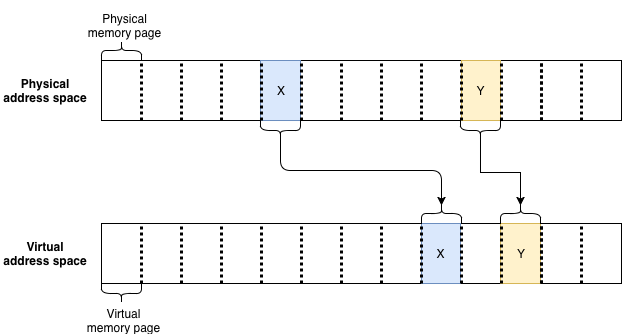
\includegraphics[width=\textwidth]{diagrams/virtual_memory.png}
	\caption{Mapping two physical memory pages X and Y to virtual memory}
	\label{fig:virtual_memory}
\end{figure}

This mapping is encoded in a data structure called the \emph{page table}. This is built up and managed by the kernel: as the application allocates and frees memory, virtual memory mappings have be created and destroyed. The representation of the page table varies depending on the architecture, but on x86-64, it can be represented as a tree, with each node an array of 512 page table entries of 8 bytes each making up a 4096 byte page table page. The root of this tree is where all virtual memory address resolution begins, and it identifies the address space. The leaf nodes are the physical memory pages that contain the application's own data.

The bits of the virtual memory address identify the page table entry to follow during address resolution. For each level of page tables, 9 bits are required to encode an index into the array of 512 entries. Each entry contains the physical memory address of the next page to traverse during the address resolution, as well as a series of bits that represent the different access permissions, such as writeable and executable. Finally, the least-significant 12 bits are used to address into the application's physical page (which is 4096 bytes) itself and so require no translation. (See Figure~\ref{fig:page_table_tree}.)

On x86-64, there are currently 4 levels of page tables, using $4 * 9 + 12 = 48$ out of the 64 available bits in the memory addresses, and limiting the size of the address space to $2^{48}$ bytes or 256 terabytes. (The size of addressable space per page table level, in reverse resolution order being: $512 * 4$ kilobytes = 2 megabytes; $512 * 2$ megabytes = 1 gigabyte; 512 gigabytes; 256 terabytes.)

\begin{figure}
	\centering
	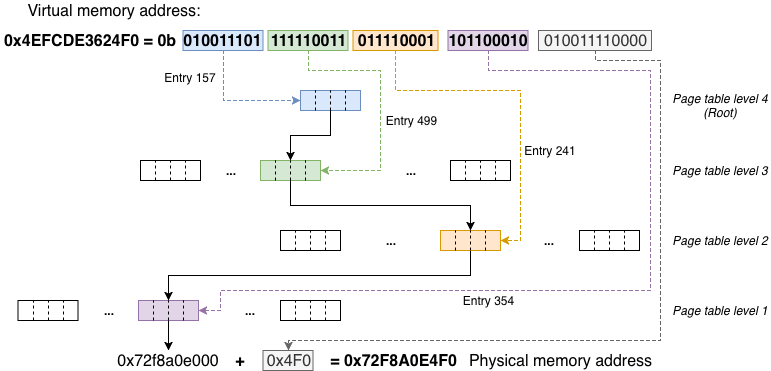
\includegraphics[width=\textwidth]{diagrams/page_table_tree.png}
	\caption{Translating a virtual memory address to physical using the page tables}
	\label{fig:page_table_tree}
\end{figure}

It's important to realize that it is possible to map a physical page into multiple virtual pages, as well as to have unmapped virtual pages. Attempting to access a virtual page (by dereferencing a pointer to it) that is not mapped -- i.e. not backed by a physical memory page -- will cause a \emph{page fault} and execution to trap inside the kernel. The kernel then can decide what to do -- for instance if it determines that the memory access was in error (an \emph{access violation}), it passes the fault on to the process which usually terminates it. On Linux this is done by raising the \texttt{SIGSEGV} signal (segmentation violation or segmentation fault) in the process, normally aborting its execution.

Other types of access violation, such as attempting to write a non-writeable page -- a page on which writing was disallowed by setting the corresponding bit in its page table entry to 0 -- or attempting to execute a non-executable page -- a page which has its no-execute bit set, a new addition in the x86-64 architecture over x86-32 -- will also trigger a page fault in the kernel the same way.

This mechanism also allows the kernel to perform memory optimizations. These are important, because (physical) memory is often a scarce resource. For example, a common scenario is that multiple running processes use the same shared library. The shared library is a single binary file on disk that is loaded into memory by multiple processes, meaning that naively the same data would be loaded into memory multiple times, taking up precious resources for no gain. The kernel can instead load the shared library into physical memory only once and then map this region into the virtual address space of each user application. Other de-duplication opportunities include static libraries that are commonly linked into applications (such as the C standard library), or the same binary executing in multiple processes.

In addition to memory de-duplication, the kernel can also choose to compress or even swap out rarely used memory. In these cases, the kernel marks the relevant page table entries as invalid, causing the hardware to trigger a page fault in the kernel if they are accessed. Upon access, instead of sending a signal to the process, the kernel restores the data by decompressing it or reading it from disk, after which it will resume the process which can continue without even being aware of what happened. Modern kernels include a large number of similar optimizations. \todo{Could probably find some citations for this}

% Thanks to Dune, Dangless has direct access to the page tables, and manipulates them using custom functions (see \textit{include/dangless/virtmem.h} and \textit{src/virtmem.c}). Upon memory allocation, Dangless forwards the allocation call to the system allocator and then reserves a new virtual page, mapping it to the same physical address as the a virtual page returned by the system allocator. This is called virtual aliasing. During deallocation, besides forwarding the call to the system allocator, Dangless unmaps the virtual alias page and overwrites the page table entry with a custom value, enabling it to recognize a would-be access through a dangling pointer.

\section{Prior art}

\todo{Oscar, etc.}

\section{Dune: light-weight process virtualization}

\todo{What is Dune, which version of Dune is used and why, and the patches applied}
\todo{Important: memory layout, how is virtual memory mapped by default, since we make extensive use of that}
\todo{Also write about how multi-threading is not currently supported by Dune, and how one could go about supporting it using the vmcall-hooks.}
\todo{Also write about the brk() bug with exceeding 4 GB leading to EPT violations; see vmcall-hooks.c}

\todo{This should probably be earlier in the chapter (or maybe in Background?)}
\todo{Also have to write about the requirements of Dangless and how to build it}

\section{Rumprun}

\todo{Development started on rumprun, why did I end up dropping it?}

\chapter{Dangless -- Implementation}
\label{ch:implementation}

\section{Initialization}
\label{sec:dangless-init}

Dangless has to be initialized before any memory allocation is performed, otherwise those allocations will not be protected. The \lstinline!REGISTER_PREINIT! option, enabled by default, controls whether Dangless should automatically register its initialization function (\lstinline!dangless_init()!) to the \lstinline!.preinit_array! section of the executable, to be called automatically during start-up.

During initialization, Dangless initializes and enters Dune by calling \lstinline!dune_init()! and \lstinline!dune_enter()!. Dangless relies on Dune to enter into a virtualized environment where it can have direct access to the page tables. Dangless also uses Dune to register its own pagefault handler function, which enables us to detect when a memory access has failed due to the protection that Dangless offers.

It's important to note that heap memory allocation can and does happen \emph{before} Dangless is initialized -- whether manually or automatically -- for example as part of the glibc runtime initialization. This case needs to be handled, so all of the \lstinline!dangless_! functions simply pass the call through to the underlying (system) allocator without doing anything else if they are called before initialization. A noteworthy edge-case that Dangless has to be able to handle is when an allocation happens before Dangless initialization, so is not protected, but then it's used and finally deallocated after initialization.

\section{Performing an allocation}

Whenever Dangless is asked to allocate some memory via a call to \lstinline!dangless_malloc()!, \lstinline!dangless_calloc()!, or \lstinline!dangless_realloc()!, a number of steps have to happen: physical memory has to be allocated, virtual memory has to be allocated, and the mapping created. Most of the process is the same regardless of the exact function called. The only exception is \lstinline!dangless_realloc()!, which I will detail later.

\subsection{Allocating physical memory}

The first step Dangelss has to perform is to acquire the physical memory it can use to satisfy the allocation. It does not currently defer allocating physical memory like kernels typically do, although in principle it could.
Since the goal of Dangless is only to provide security benefits, Dangless has no strategy of physical memory management unlike normal implementations. In fact, the way this is done ultimately does not matter for Dangless' purposes. Due to these reasons, Dangless delegates the responsibility of actually performing (physical) memory allocation to the memory allocator that was in place before Dangless "hijacked" the memory management function symbols.

Specifically, it uses \lstinline!dlsym(RTLD_NEXT, "malloc")! to determine the address of the original \lstinline!malloc()!, etc. functions. Then it simply calls these functions whenever it needs physical memory allocation done: primarily when the user code requests an allocation, but sometimes also for internal purposes, such as for keeping track of available virtual memory regions.

There is a caveat to using \lstinline!dlsym()!: when \lstinline!dlsym()! it is first called on a thread, it allocates a thread-specific buffer for holding a \lstinline!struct dl_action_result! object using \lstinline!calloc()!~\cite{glibc-dlsym-calls-calloc}. This means that without special handling for this case, execution can easily get into an infinite loop:

\begin{enumerate}
	\item User calls \lstinline!malloc()!, which is a strong alias of \lstinline!dangless_malloc()!
	\item \lstinline!dangless_malloc()! defers the physical memory allocation to the underlying allocator by calling \lstinline!sysmalloc()!
	\item \lstinline!sysmalloc()! does not yet have the address of the original \lstinline!malloc()! function, so it calls \lstinline!dlsym()! to get it
	\item \lstinline!dlsym()! notices it's running on this thread for the first time, so it calls \lstinline!calloc()! to allocate a buffer
	\item \lstinline!calloc()! is a strong alias of \lstinline!dangless_calloc()!, which calls \lstinline!syscalloc()! to allocate physical memory
	\item \lstinline!syscalloc()! does not yet have the address of the original \lstinline!calloc()! function, so it calls \lstinline!dlsym()!
	\item Repeat steps 4-6 forever...
\end{enumerate}

To get around this, \lstinline!syscalloc()! uses a static buffer of \lstinline!CONFIG_CALLOC_SPECIAL_BUFSIZE! size for the very first allocation. This allows \lstinline!dlsym()! to complete and populate the addresses of the original allocation functions, which are used normally for all subsequent calls. The same approach was used by other projects that implement their own memory allocator replacements~\cite{dlsym-calloc-special-ex1}.

Finally, when \lstinline!sysmalloc()!, etc. returns, we have a completed physical memory allocation. However, what is returned to us is a virtual memory address. We could perform a pagetable walk to find the corresponding physical memory address, but this is unnecessary, as the mapping provided by Dune is very simple, so it's sufficient to use Dune's \lstinline!dune_va_to_pa()! function from \texttt{libdune/dune.h} that is far cheaper computationally than a page-table walk.

The implementation of Dangless cannot handle the system allocator returning a (guest) virtual memory region that is backed by non-contiguous (guest) physical memory. This should not normally be a problem, unless Dangless is used together with code that implements the system calls used by memory allocators (usually \lstinline!brk()! and \lstinline!mmap()!).
Note that it does not matter whether the host physical memory is contiguous or not: any \lstinline!mmap()! (or \lstinline!brk()! for that matter) allocation is mapped into the guest memory contiguously. \todo{I think that's the case though, but I'm not totally sure. Check this? Note that the implementation can be fixed if necessary.}

\subsection{Allocating virtual memory}
\label{sec:dangless-alloc-virtmem}

Given a physical memory address of the user allocation, Dangless needs to allocate the same amount of virtual memory pages that user code will interact with. In the memory layout created by Dune, there's plenty of virtual memory that is not used, nor will ever be used normally due to the size limitations of the various memory regions that Dune enforces.

For simplicity, and in order to minimize the chance of conflicts, by default Dangless upon the first memory allocation request that it can't satisfy due to not having sufficient virtual memory, will take any unused entries from the top-level page table (PML4)  and initialize its virtual memory allocator with them marked as available. This behaviour can be disabled using the \lstinline!AUTO_DEDICATE_PML4ES! option. Users can also dedicate virtual memory to Dangless using the \lstinline!dangless_dedicate_vmem(void *start, void *end)! function (declared in \texttt{dangless\_malloc.h}).

The amount of virtual memory available to Dangless has to be very large, as each allocation will use up at least one whole 4 KB page from it. This is done so that during deallocation the page can be marked as unmapped in order to cause any further accesses to it fail. (The most precise level of granularity it is possible to do this on x86-64 based systems today is the 4 KB page.) This means that 1 GB of virtual memory can be used to satisfy $1 GB / 4 KB = 256 * 1024 = 262 144$ allocations, assuming each of them is less than 4 KB in size. This is because currently Dangless lacks any mechanisms for detecting that a virtual memory region is no longer referenced, meaning that it will never mark a virtual memory page as available for reuse.

To keep track of the virtual memory available to it, Dangless employs a simple freelist-based span allocator. A freelist is simply a singly linked-list of \lstinline!vp_span! objects each representing a free span of virtual memory, ordered by their end address:

\begin{lstlisting}
struct vp_span {
	vaddr_t start;
	vaddr_t end;
	
	LIST_ENTRY(vp_span) freelist;
};

struct vp_freelist {
	LIST_HEAD(, vp_span) items;
};
\end{lstlisting}

(The NetBSD \texttt{queue.h}~\cite{netbsd-queue-ref} v1.68 is used for the linked list handling macros.)

When virtual memory is needed, the freelist is walked until a \lstinline!vp_span! object representing a region of sufficient size is found. When one is found, the allocated space is removed from the beginning of the span (by adjusting \lstinline!start!), and the span is deleted if it is now empty. If no such span is found, the allocation fails.

When an allocation fails, Dangless checks if it's allowed to auto-dedicate virtual memory by consulting the \lstinline!AUTO_DEDICATE_PML4ES! option. If this option is enabled, and Dangless hasn't yet done so, it will proceed to do this before re-trying the allocation.

Otherwise, Dangless concludes that it's unable to satisfy the user's memory allocation. If \lstinline!ALLOW_SYSMALLOC_FALLBACK! is enabled (defaults to off), then Dangless proceeds by simply acting as a proxy to the system allocator, and gives up on attempting to protect the allocation. Otherwise, Dangless prints an error message and terminates the application.

Note that in the current, simple implementation of the virtual memory allocator there is only a single freelist, which is sufficient because we do not ever re-use any virtual memory. If we were to add a garbage collector-like solution, then this approach would likely lead to significant fragmentation with a negative performance impact on each allocation. In this situation, a possible enhancement would be to have several independent freelists of different page sizes, similar to common memory allocator designs. Other improvements are also possible: memory allocation is a well-understood problem.

\subsection{Remapping}

\todo{Use diagrams for this, such as the ones used in the presentation}

Now that Dangless has the physical memory address and a brand new virtual memory address, all that is left to do is mapping the virtual memory to the physical memory by modify the corresponding page table.

In a normal Linux userland application, in order to do this we would have to perform a system call, given that page table manipulation requires ring 0 privileges meaning that it's only available to the kernel. However, thanks to Dune, the process is running inside its own virtualized environment, in which we can act as the kernel, and for instance read control register 3 (\lstinline!cr3!) containing the (guest) physical address of the page table root.

Having applied the \texttt{dune-ix-guestppages.patch} patch to Dune, the host memory pages used to hold the guest's page tables are mapped into the guest virtual memory, allowing us to manipulate them during runtime from inside the guest environment.

\subsection{Deallocations}
\label{ssec:deallocations}

When deallocating some memory using \lstinline!dangless_free()!, the challenge is detecting whether the given pointer was successfully remapped previously, and if so, obtaining the original virtual address that can be passed to \lstinline!sysfree()!.
This is necessary if we don't want to make assumptions about the underlying allocator's implementation details. Typically, memory allocators will not behave correctly if a different virtual memory address is used for deallocation than the one returned during allocation, even if both map to the same physical memory address.

To obtain the original virtual memory address, we make use of Dune's simple memory layout. First, we perform a page walk on the virtual memory address to obtain the corresponding physical memory address. Then we can compare \lstinline!dune_va_to_pa(ptr)! (where \lstinline!ptr! is the potentially-remapped memory address we're trying to free) to the resulting physical address.
If they match, then \lstinline!ptr! was mapped into virtual memory by Dune itself, meaning that it's not a memory address assigned by Dangless. This is possible, on allocations that were performed before Dangless finished initializing. In this case, we can simply call \lstinline!sysfree()! to perform the deallocation.

Otherwise, we have to determine what Dune-mapped virtual memory address belongs to the obtained physical memory address. In other words, given \lstinline!PA!, we have to determine \lstinline!VA! such that \lstinline!dune_va_to_pa(VA) = PA!. Once again, this is something that Dune's memory layout makes easy to do, as these conversions are performed using simple arithmetic. Finally, we can call \lstinline!sysfree()! to perform the physical memory deallocation.

What is left to do is invalidating the page table entries for the remapped virtual memory address, to make sure that any dangling pointer access will fail. Locating the relevant page table entries is done by performing a page-table walk down to the 4K pages. The relevant page table entries are then overwritten by an entry that does not have the \emph{present} bit set. Dangless uses the 64-bit value \lstinline!0xDEAD00! for this purpose, to make the invalidated entries easily identifiable. We then flush the TLB (Translation Lookaside Buffer; used to cache the results of pagewalks for performance) to force the CPU to check the PTE should an access occur.

In order to determine how many of the page table entries we need to invalidate, we have to know how many 4K pages did the allocation span. Recall that Dangless places each allocation on virtual memory pages that will never be used for anything else. \lstinline!malloc_usable_size()! is used to get the size of the allocation in bytes. (Of course, this has to be done before calling \lstinline!sysfree()!.) Note though that determining the number of spanned pages is not as easy as it might seem at the first glance, because the allocation can start anywhere within a memory page. This means that, for instance a 512-byte region can span 1 or 2 pages depending on where it begins within the first page (Figure~\ref{fig:allocation-spanned-pages}).

\begin{figure}
	\centering
	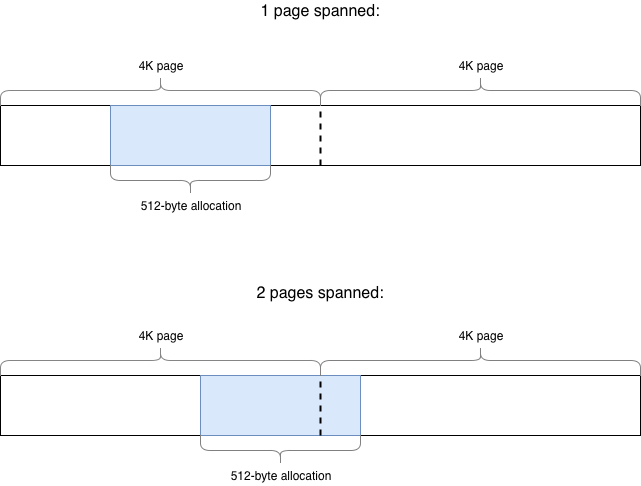
\includegraphics[width=\textwidth]{diagrams/allocation_spanned_pages.png}
	\label{fig:allocation-spanned-pages}
	\caption{A memory allocation can span different number of pages depending on where it begins}
\end{figure}

\subsection{Handling realloc}
\todo{Is this interesting to write about? It's just a software engineering problem, nothing theoretically interesting about it}

%The standard \lstinline!realloc()! function has more complicated behaviour. For instance, \lstinline!realloc(NULL, some_size)! is valid and equivalent to calling \lstinline!malloc(some_size)! in order to simplify user code. Next, Dangless needs to be able the cases both when the original came from Dangless (so is a remapped pointer), and when it did not. For instance, it's possible that the original pointer came from an allocation before Dangless finished initializing, or was created when Dangless did not have available virtual memory to perform remapping.
%
%In order to determine whether the original pointer was remapped or not, we use the same logic as during \lstinline!dangless_free()!: perform a page-table walk to get the backing physical address and then check whether the received pointer is one that would be generated by Dune when mapping its memory layout by checking the result of \lstinline!dune_pa_to_va()!. If we find that it's not a remapped pointer, then for the purposes of Dangless, this is a new allocation: simply forward the call to \lstinline!sysrealloc()! and remap the resulting pointer.
%
%Otherwise, the situation is more complicated. We have to handle the case when \lstinline!sysrealloc()! performed an in-place resize.

\section{Fixing up vmcalls}
\label{sec:vmcall-pointer-rewriting}

\subsection{The problem}

One of the goals of Dune is to remain as simple as possible, and not re-implement most functionality of operating system kernels when not absolutely necessary. This means that most system calls performed the application running inside Dune are not actually handled by Dune itself, but rather are passed on to the host kernel via the \lstinline!vmcall! instruction. (\lstinline!vmcall! is identical to \lstinline!syscall!, except it exits the virtual environment first.) This includes tasks as common as I/O operations (such as \lstinline!printf()! or \lstinline!fopen()!), or even memory management (such as \lstinline!mmap()!).

This presents a challenge for Dangless, which can be efficient because it can directly manipulate the page tables inside the virtual environment (guest machine) itself, without having to manipulate the host's page tables (which would only be possible via a system call such as \lstinline!mprotect()!). However, any virtual memory addresses returned from Dangless will only be valid inside the guest environment, meaning that attempting to pass such a memory address to the host kernel when performing a system call (vmcall) will fail with \lstinline!EINVAL!.

To demonstrate the problem, first consider the following:

\begin{lstlisting}
puts("Hello world!\n");
\end{lstlisting}

The \lstinline!puts()! standard library function used here is a comparatively simple wrapper around the \lstinline!write()! system call, and unlike \lstinline!printf()!, does not perform any formatting or other manipulation of the string~\cite{glibc-puts-analysis}. Recall that in C, strings are represented by null-terminated character arrays, and are typically passed to functions as \lstinline!const char*!: a (virtual) memory address pointing to the first character of the string. Since in this example, the argument to \lstinline!puts()! is a string literal, the string data is stored in the executable's data section (such as \texttt{.rodata}) without any dynamic memory allocation that would go through Dangless. The result is that the pointer passed to the \lstinline!write()! vmcall references virtual memory that is mapped by the host machine, so the call will succeed.

\begin{lstlisting}
void determineAnswer(char* buffer) {
	strcpy(buffer, "Fourty-two");
}

char* answerBuffer = malloc(64 * sizeof(char));
determineAnswer(answerBuffer);

puts("The answer is: ");
puts(answerBuffer);
puts("\n");

free(answerBuffer);
\end{lstlisting}

I hope that the problem is now clear: we're passing a \lstinline!malloc()!-d buffer to \lstinline!puts()!. Since \lstinline!malloc()! refers to \lstinline!dangless_malloc()!, it will perform virtual memory remapping inside the guest system, yielding a pointer value in \lstinline!answer! that is valid inside the guest machine, but not in the host machine. (Of course, the data is present in the host physical memory, but is not mapped to host virtual memory.) The \lstinline!write()! system call when executed by the host, is not going to be amused by this fact, and is going to return the error code \texttt{EINVAL}, indicating an invalid argument.

In this case by knowing how Dangless works it is easy to spot the problem. However, often dynamic memory allocation is performed and the resulting pointer is passed to a system call in a way that's not immediately obvious from the user code, such as when done internally by the standard library implementation. The simplest example is probably \lstinline!printf()!, which can call \lstinline!malloc()! in some circumstances~\cite{glibc-printf-malloc}~\cite{glibc-printf-malloc-vulnerability}. I've also already mentioned how \lstinline!dlsym()! when running for the first time will call \lstinline!calloc()!.

\subsection{Intercepting vmcalls}

In order to fix this problem, Dangless needs to intercept any system calls that are about to be forwarded to the host kernel. This capability is not provided by default in Dune, so I've implemented it (\texttt{dune-ix-vmcallhooks.patch}), allowing Dangless to register a pre- and post-hook function that will be called before and after a \lstinline!vmcall! instruction is performed by Dune, respectively. In the pre-hook, Dangless can access and modify the system call number, any of the arguments, and even the return address. Similarly, the post-hook exposes the syscall return code.

\subsection{Determining which arguments to rewrite}

The next problem is how to determine what the system call arguments are, and which of them can possibly reference a Dangless-remapped pointer. Note that it is not sufficient to find the pointers among the arguments themselves, as pointers can be nested: the arguments can be pointers to arrays or structures which in turn contain pointers -- sometimes, after a few layers of indirection. Examples include the \lstinline!readv()! and \lstinline!writev()! system calls, which are used by GNU implementation of the \lstinline!<iostream>! standard C++ header such as when writing to \lstinline!std::cout!, i.e. \lstinline!stdout!:

\begin{lstlisting}
ssize_t readv (int fd, const struct iovec *v, int n);
ssize_t writev(int fd, const struct iovec *v, int n);

struct iovec {
	void  *iov_base; /* Starting address */
	size_t iov_len;  /* Number of bytes */
};
\end{lstlisting}

When handling either of these functions, not just the \lstinline!const struct iovec *v! pointer has to be fixed, but also the \lstinline!void *iov_base! pointer inside the pointer \lstinline!struct iovec!.

Another example is the functions \lstinline!execve()! and \lstinline!execveat()!:

\begin{lstlisting}
int execve(const char *filename, char *const argv[], char *const envp[]);
int execveat(int dirfd, const char *pathname, char *const argv[], char *const envp[], int flags);
\end{lstlisting}

Besides the \lstinline!const char *filename! simple pointer, the parameters \lstinline!char *const argv[]! and \lstinline!char *const envp[]! are both a null-terminated array of pointers, in which every entry has to be fixed.

Finally, pointers to more complicated structures are also sometimes passed as system call arguments:

\begin{lstlisting}
ssize_t recvmsg(int sockfd, struct msghdr *msg, int flags);

struct msghdr {
	void         *msg_name;       /* optional address */
	socklen_t     msg_namelen;    /* size of address */
	struct iovec *msg_iov;        /* scatter/gather array */
	size_t        msg_iovlen;     /* # elements in msg_iov */
	void         *msg_control;    /* ancillary data, see below */
	size_t        msg_controllen; /* ancillary data buffer len */
	int           msg_flags;      /* flags on received message */
};
\end{lstlisting}

So, we need some way to determine which arguments of the system call can be a pointer, and identify what data structure it points to in order to find any nested pointers. Essentially, what we need is to be able to tell for a system call number what arguments it takes and what type they are. For this purpose, I have created a Python module \texttt{linux-syscallmd} (source on GitHub~\cite{github-linux-syscallmd}) that parses the Linux kernel header file \texttt{include/linux/syscalls.h} and exposes system call metadata to user code. The Dangless script at \texttt{make/gen\_vmcall\_fixup\_info.py} then uses this information to generate a file containing C code that can be \lstinline!#include!-d to utilize this data inside Dangless:

\begin{lstlisting}
// sources/src/platform/dune/vmcall_fixup_info.h

enum vmcall_param_fixup_type {
	VMCALL_PARAM_NONE,
	VMCALL_PARAM_FLAT_PTR,
	VMCALL_PARAM_IOVEC,
	VMCALL_PARAM_PTR_PTR,
	VMCALL_PARAM_MSGHDR
}

struct vmcall_param_fixup_info {
	enum vmcall_param_fixup_type fixup_type;
};

struct vmcall_fixup_info {
	i8 num_params;
	struct vmcall_param_fixup_info params[SYSCALL_MAX_ARGS];
};

// sources/src/platform/dune/vmcall_fixup_info.c

static const struct vmcall_fixup_info g_vmcall_fixup_info_table[] = {
	// generated by make/gen_vmcall_fixup_info.py
	#include "dangless/build/common/vmcall_fixup_info.inc"
};
\end{lstlisting}

The generated array is indexed by the number of a system call to find its corresponding entry. Then we can iterate through the arguments and act on them based on the \lstinline!enum vmcall_param_fixup_type! value.

As an example, the entry for the \lstinline!clone()! system call looks like this:

\begin{lstlisting}
static const struct vmcall_fixup_info s_clone_info = {
	.num_params = 5,
	.params = {
		// unsigned long flags
		[0] = {
			.fixup_type = VMCALL_PARAM_NONE
		},
		
		// void *child_stack
		[1] = {
			.fixup_type = VMCALL_PARAM_FLAT_PTR
		},
		
		// int *ptid
		[2] = {
			.fixup_type = VMCALL_PARAM_FLAT_PTR
		},
		
		// int *ctid
		[3] = {
			.fixup_type = VMCALL_PARAM_FLAT_PTR
		},
		
		// unsigned long newtls
		[4] = {
			.fixup_type = VMCALL_PARAM_NONE
		}
	}
};
\end{lstlisting}

\subsection{Rewriting the pointers}

Now that we know which arguments to rewrite or "fix-up", we can use the same logic as \lstinline!dangless_free()! to get the canonical pointer from a potentially-remapped one (see Section~\ref{ssec:deallocations}). We then replace the remapped pointer value with the canonical one in the system call arguments.

In case of nested pointers this involves modifying the referenced in-memory data, meaning we cannot simply replace the pointer. This is because the original pointer was a remapped pointer, allocated via Dangless, and will be deallocated via Dangless. However, due to the nested pointer fix-up, the user code can now potentially access the canonical (non-remapped) pointer, opening the door to dangling pointer errors. Furthermore, should a canonical pointer be passed to \lstinline!dangless_free()!, it cannot invalidate the remapped memory region as it doesn't know where it might be.

To demonstrate, consider the following code:

\begin{lstlisting}
char *first = malloc(32);
strcpy(first, "Hello ");

char *second = malloc(32);
strcpy(second, "world!");

struct iovec iov[2];
iov[0].iov_base = first;
iov[0].iov_len = strlen(first);
iov[1].iov_base = second;
iov[1].iov_len = strlen(second);

writev(STDOUT_FILENO, iov, 2);
\end{lstlisting}

Due to pointer rewriting the system call succeeds, but afterwards we end up with \lstinline|iov[0].iov_base != first| and \lstinline|iov[1].iov_base != second|, as they have been replaced by their canonical counterparts to make the system call succeed on the host kernel.

Later, we deallocate the buffers:

\begin{lstlisting}
free(second);
free(first);
\end{lstlisting}

This is fine, since the \lstinline!first! and \lstinline!second! variables were not affected by the pointer rewriting, so Dangless correctly invalidates the remapped regions in \lstinline!dangless_free()!. But then, later:

\begin{lstlisting}
fprintf(stderr, "Attempted writev() with '%s' and '%s'!\n", iov[0].iov_base, iov[1].iov_base);
\end{lstlisting}

Here we have an attempted memory access through two dangling pointers. Recall that, due to pointer rewriting, \lstinline|iov[0].iov_base| and \lstinline|iov[1].iov_base| are the canonical pointers (as returned by \lstinline!sysmalloc()!) and so do not point into the remapped region that was invalidated by the earlier \lstinline!dangless_free()! calls. Therefore, this error will not be caught by Dangless!

To resolve this situation, for every nested pointer fix-up, Dangless records the pointer location (a pointer to the user pointer) as well as the original value stored there (the Dangless-remapped pointer value) in a buffer. After the vmcall returns but before it jumps back into user code, we then go through the records and restore any such rewritten pointer values to their original ones, preventing the user from being exposed to non-remapped pointer values.

\subsection{Limitations}

This approach is limited in that Dangless can only handle system calls, arguments, and argument types that \texttt{linux-syscallmd} recognizes when building Dangless.

For instance, \texttt{linux-syscallmd} currently does not understand or process preprocessor macros, such as \lstinline!#if! and \lstinline!#ifdef! sections. This means that system call signatures not relevant for the current system will also be parsed, leading to conflicting signatures for some system calls, such as \lstinline!clone()!. \texttt{linux-syscallmd} currently does not handle this situation, and will just pick the last occurrence of the same system call in the source file, which may be different than the signature actually used by the kernel. Because of this, Dangless has special handling of the \lstinline!clone()! system call, but naturally that can't extend to e.g. system calls introduced in the future.

As of writing, I do not know of a better way to approach this. Fixing the present limitation would involve knowing what values were used for each preprocessor macro while building the kernel, and I'm not aware of any way in which the kernel exposes this information.

Another issue is understanding which arguments can hold pointer or nested pointer values. For the vast majority of system calls this is straight-forward, as \texttt{linux/syscall.h} consistently marks the pointer arguments as \lstinline!__user *!, and the pointed type is obvious, whether it's \lstinline!char! or \lstinline!struct iovec!. But some system calls will interpret the same argument differently depending on the context of the call, such as \lstinline!ptrace()!. The signature of \lstinline!ptrade()! is as follows:

\begin{lstlisting}
long ptrace(enum __ptrace_request request, pid_t pid, void *addr, void *data);
\end{lstlisting}

Notice that \lstinline!addr! and \lstinline!data! are both untyped (\lstinline!void!) pointers. How they are interpreted differs depending on the value of the \lstinline!request! argument. Some examples:

\begin{itemize}
	\item \lstinline!PTRACE_TRACEME!: both \lstinline!addr! and \lstinline!data! are ignored.
	\item \lstinline!PTRACE_PEEKTEXT!: \lstinline!addr! does \emph{not} correspond to pointer in the address space of the caller, but rather, refers to a location in the address space of the target application. The same pointer value may reference a memory region that's unmapped, or worse, mapped for something completely different in the address space of the calling process. As such, Dangless should not touch it. \lstinline!data! is ignored.
	\item \lstinline!PTRACE_POKEDATA!: \lstinline!addr! refers to a memory address in the target process. \lstinline!data! might not be a pointer value at all, but rather the word to be copied into the target process' memory.
	\item \lstinline!PTRACE_GETREGS!: \lstinline!data! is an actual pointer in the calling process, while \lstinline!addr! is ignored.
	\item \lstinline!PTRACE_GETREGSET!: \lstinline!addr! is not a pointer value at all, but rather an enumeration. \lstinline!data! is an actual pointer to the calling process' memory, but it references a \lstinline!struct iovec! value, meaning that it will contain nested pointers that also have to be fixed up by Dangless.
\end{itemize}

\lstinline!ptrace()! is a special case due to its very specialized nature, and it's unlikely to be used at all in the vast majority of applications that Dangless would be relevant for. Because of this Dangless ignores \lstinline!ptrace()!, even though it would be possible to cover all of these scenarios.

There may be other system calls that have similar behaviour, although likely not as pathological as \lstinline!ptrace()!. These are currently not handled in any way by texttt{linux-syscallmd} nor Dangless. Supporting all of these scenarios would inevitably involve extending Dangless to handle each on a case-by-case basis.

\todo{Probably have a chapter about using Dangless, such as how to build Dangless, what system requirements does it have, and how to make it work on an existing application.}

\chapter{User guide}
\label{ch:user-guide}

This chapter is about building, configuring, and using Dangless.
Most of this information in less detail is also described in the repository \path{README} file.

\section{System requirements}

Most requirements are posed by Dune itself:

\begin{itemize}
	\item A 64-bit x86 Linux environment
	\item A relatively recent Intel CPU with VT-x support
	\item Kernel version of 4.4.0 or older
	\item Installed kernel headers for the running kernel
	\item Root (sudo) privileges
	\item Enabled and sufficient number of hugepages (see below)
\end{itemize}

The remaining requirements posed by Dangless itself are fairly usual:

\begin{itemize}
	\item A recent C compiler that supports C11 and the GNU extensions (either GCC or Clang will work)
	\item Python 3.6.1 or newer
	\item CMake 3.5.2 or newer
\end{itemize}

\subsection{Hugepages}

Besides the above, Dune requires some 2 MB hugepages to be available during initialization for setting up its safe stacks. It will also try to use huge pages to acquire memory for the guest's page allocator, although it will gracefully fall back if there are not enough huge pages available.

To make sure that some huge pages remain available, it is recommended to limit or disable transparent hugepages by setting \path{/sys/kernel/mm/transparent_hugepage/enabled} to \emph{madvise} or \emph{never} (you will need to use \path{su} if you want to change it).

Then, you can check the number of huge pages available:

\begin{lstlisting}[breaklines, language=, style=]
$ cat /proc/meminfo | grep Huge
AnonHugePages:     49152 kB
HugePages_Total:     512
HugePages_Free:      512
HugePages_Rsvd:        0
HugePages_Surp:        0
Hugepagesize:       2048 kB
\end{lstlisting}

In my tests, it appears that at minimum \textbf{71} free huge pages are required to satisfy Dune, although it is not quite clear to me as to why: by default for 2 safe stacks of size 2 MB each, we should only need 2 hugepages.

You can dedicate more huge pages by modifying \path{/proc/sys/vm/nr_hugepages} (again, you will need to use \texttt{su} to do so), or by executing:

\begin{lstlisting}[breaklines, language=, style=]
sudo sysctl -w vm.nr_hugepages=<NUM>
\end{lstlisting}

... where \texttt{<NUM>} should be replaced by the desired number, of course.

When there is not a sufficient number of huge pages available, Dangless will fail while trying to enter Dune mode, and you will see output much like this:

\begin{lstlisting}[breaklines, language=, style=]
dune: failed to mmap() hugepage of size 2097152 for safe stack 0
dune: setup_safe_stack() failed
dune: create_percpu() failed
Dangless: failed to enter Dune mode: Cannot allocate memory
\end{lstlisting}

\section{Building and configuring}

The full Dangless source code is available on GitHub at \url{https://github.com/shdnx/dangless-malloc}. After cloning, you will have to start by setting up its dependencies (such as Dune) which are registered as git submodules in the \path{vendor} folder:

\begin{lstlisting}[breaklines, language=bash, style=]
git submodule init
git submodule update
\end{lstlisting}

Then we have to apply the Dune patches as described in Section~\ref{sec:bg-dune} and build it:

\begin{lstlisting}[breaklines, language=bash, style=]
cd vendor/dune-ix

# patch dune, so that the physical page metadata is accessible inside the guest, allowing us to e.g. mess with the pagetables
git apply ../dune-ix-guestppages.patch

# patch dune, so that we can register a prehook function to run before system calls are passed to the host kernel
git apply ../dune-ix-vmcallprehook.patch

# patch dune, so that it does not kill the process with SIGTERM when handling the exit_group syscall - this causes runs to be registered as failures when they succeeded
git apply ../dune-ix-nosigterm.patch

# need sudo, because it is building a kernel module
sudo make
\end{lstlisting}

Now configure and build Dangless using CMake:

\begin{lstlisting}[breaklines, language=bash, style=]
cd ../../sources

mkdir build
cd build

# you can specify your configuration options here, or e.g. use ninja (-GNinja) instead of make
cmake \
	-D CMAKE_BUILD_TYPE=Debug \
	-D OVERRIDE_SYMBOLS=ON \
	-D REGISTER_PREINIT=ON \
	-D COLLECT_STATISTICS=OFF \
	..

cmake --build .
\end{lstlisting}

You should be able to see \path{libdangless_malloc.a} and \path{dangless_user.make} afterwards in the build directory.

You can see what configuration options were used to build Dangless by listing the CMake cache:

\begin{lstlisting}[breaklines, language=C, style=]
$ cmake -LH
-- Cache values
// Whether to allow dangless to gracefully handle running out of virtual memory and continue operating as a proxy to the underlying memory allocator.
ALLOW_SYSMALLOC_FALLBACK:BOOL=ON

// Whether Dangless should automatically dedicate any unused PML4 pagetable entries (large unused virtual memory regions) for its virtual memory allocator. If disabled, user code will have to call dangless_dedicate_vmem().
AUTODEDICATE_PML4ES:BOOL=ON

// Choose the type of build, options are: None(CMAKE_CXX_FLAGS or CMAKE_C_FLAGS used) Debug Release RelWithDebInfo MinSizeRel.
CMAKE_BUILD_TYPE:STRING=Debug

// Install path prefix, prepended onto install directories.
CMAKE_INSTALL_PREFIX:PATH=/usr/local

// Whether to collect statistics during runtime about Dangless usage. If enabled, statistics are printed after every run to stderr. These are only for local developer use and are not uploaded anywhere.
COLLECT_STATISTICS:BOOL=OFF

// Debug mode for dangless_malloc.c
DEBUG_DGLMALLOC:BOOL=OFF

// Debug mode for vmcall_fixup.c
DEBUG_DUNE_VMCALL_FIXUP:BOOL=OFF
...
\end{lstlisting}

You can also use a CMake GUI such CCMake~\cite{ccmake-website}, or check the main CMake file (\path{sources/CMakeLists.txt}) for the list of available configuration options, their description and default values.

\section{API overview}

Dangless is a Linux static library \path{libdangless_malloc.a} that can be linked to any application during build time. It defines a set of functions for allocating and deallocating memory:

\begin{lstlisting}
// sources/include/dangless/dangless_malloc.h

void *dangless_malloc(size_t sz) __attribute__((malloc));
void *dangless_calloc(size_t num, size_t size) __attribute__((malloc));
void *dangless_realloc(void *p, size_t new_size);
int dangless_posix_memalign(void **pp, size_t align, size_t size);
void dangless_free(void *p);
\end{lstlisting}

These functions have the exact same signature and behaviour as their standard counterparts \lstinline!malloc()!, \lstinline!calloc()!, and \lstinline!free()!. In fact, because the GNU C Library defines these standard functions as weak symbols~\cite{glibc-malloc-is-weak}, Dangless provides an option (\lstinline!OVERRIDE_SYMBOLS!) to override the symbols with its own implementation, enabling the user code to perform memory management without even being aware that it is using Dangless in the background.

Besides the above, Dangless defines a few more functions, out of which the following two are important.

\begin{lstlisting}
void dangless_init(void);
\end{lstlisting}

Initializes Dangless as described in Section~\ref{sec:dangless-init}. Whether or not this function is called automatically during application start-up is controlled by the \lstinline!REGISTER_PREINIT! option, defaulting to On.

\begin{lstlisting}
int dangless_dedicate_vmem(void *start, void *end);
\end{lstlisting}

Dedicates a memory region to Dangless's virtual memory allocator, as described in Section~ref{sec:dangless-alloc-virtmem}.
Whether or not any dedication happens automatically is controlled by the \lstinline!AUTO_DEDICATE_PML4ES! option.

\section{Integrating into existing applications}

Dangless can be integrated into an application which relies, directly or indirectly, the C memory management API. To do this:
\begin{itemize}
	\item link to \path{libdangless_malloc.a} using the \texttt{--whole-library} option
	\item link to \path{libdune.a}
	\item link to \path{libdl} to allow Dangless to resolve the symbols for the system allocator
	\item disable building a position-independent executable (PIE) using \texttt{-no-pie}, due to the limitation of Dune
\end{itemize}

When building, Dangless generates a \path{dangless_user.make} file that makes this easier to do with Makefile-based build systems.

\chapter{Evaluation}

\section{Performance on SPEC 2006}

All measurements were made on Intel Core i7-4510U CPU @ 2.00GHz with 16 GB RAM, running Ubuntu 14.04 LTS, with Linux kernel version 4.4.0-161. Performance overhead was measured on the standard SPEC2006 benchmarking suite using the VUSec group's \texttt{instrumentation-infra} framework~\cite{vusec-infra}.

Dangless was built and configured in the following manner:

\begin{lstlisting}[breaklines, language=bash, style=]
./setup.py build \
	--dangless-config ALLOW_SYSMALLOC_FALLBACK=Off \
	--dangless-config COLLECT_STATISTICS=Off \
	--dangless-config ENABLE_PERF_EVENTS=Off \
	--dangless-config REPORT_RUSAGE=Off \
	--dangless-config SYSCALLMETA_HAS_INFO=Off \
	--targets spec2006 \
	--instances baseline dune-only dangless-malloc
\end{lstlisting}

This builds SPEC2006 in three configurations (referred to as ``instances''):
\begin{enumerate}
	\item \emph{baseline}: plain, unmodified benchmarks.
	\item \emph{dune-only}: all benchmarks are built linking to \path{libdune}, as well as a small utility library ensuring that Dune is entered automatically at program startup (\path{libdune-autoenter}). This is used to measure the overhead of Dune itself compared to \emph{baseline}.
	\item \emph{dangless-malloc}: linking to \path{libdangless-malloc} and its dependencies, measuring the overhead of Dangless itself.
\end{enumerate}

The above command line corresponds to building Dangless manually like so:

\begin{lstlisting}[breaklines, language=bash, style=]
cmake \
	-D CMAKE_BUILD_TYPE=RelWithDebInfo \
	-D ALLOW_SYSMALLOC_FALLBACK=Off \
	-D COLLECT_STATISTICS=Off \
	-D ENABLE_PERF_EVENTS=Off \
	-D REPORT_RUSAGE=Off \
	-D SYSCALLMETA_HAS_INFO=Off \
	..

cmake --build .
\end{lstlisting}

Finally, the benchmarks were run using the command:

\begin{lstlisting}[breaklines, language=bash, style=]
./setup.py run \
	--parallel=proc \
	--parallelmax=1 \
	--iterations=5 \
	spec2006 \
	baseline \
	dune-only \
	dangless-malloc \
	--benchmarks all_c all_cpp
\end{lstlisting}

This runs all of the C and C++ SPEC2006 benchmarks in all three configurations, sequentially (\texttt{parallelmax=1}), 5 times each.

Dangless successfully runs on all C and C++ benchmarks with following exceptions:

\begin{itemize}
	\item \path{400.perlbench} with test workload fails due to using the unsupported \lstinline!clone()! system call
	\item \path{400.perlbench} and \path{471.omnetpp} with reference workload both fail in very similar circumstances, indicating an EPT violation error. It is not clear what the cause is, but I suspect it is some limitation or bug in Dune.
\end{itemize}

\todo{So both benchmarks in ref workload fail with GPA = GVA = 0x2801ff000. Dune's PAGEBASE starts at 0x200000000. Does it maybe get overwritten after heap allocations? Test it!}

The performance overhead results are summarized in Table~\ref{tab:perf-dune-dangless-oscar} and visualized in Figure~\ref{fig:perf-dune-dangless-oscar}. Memory overhead results are summarized in Table~\ref{tab:mem-dune-dangless-oscar} and visualized in Figure~\ref{fig:mem-dune-dangless-oscar}. For comparison, I have included the overheads from Oscar~\cite{oscar2017}, which represents the current state of the art. Because unfortunately they have not published the exact numbers, these are estimations based on their included graphs.

% Performance overhead: Dune vs Dangless vs Oscar
\begin{table}[]
	\centering
	\begin{tabular}{|l|l|l|l|}
		\hline
		\textbf{Benchmark} & \textbf{Dune} & \textbf{Dangless} & \textbf{Oscar} \\ \hline
		401.bzip2          & 0.995         & 1.013             & 1.000                      \\ \hline
		403.gcc            & 0.987         & 1.152             & 1.250                      \\ \hline
		429.mcf            & 1.003         & 1.115             & 1.000                      \\ \hline
		433.milc           & 1.039         & 1.107             & 1.055                      \\ \hline
		444.namd           & 1.000         & 1.004             & 1.000                      \\ \hline
		445.gobmk          & 1.001         & 1.025             & 1.005                      \\ \hline
		447.dealII         & 1.008         & 1.074             & 2.900                      \\ \hline
		450.soplex         & 1.004         & 1.030             & 1.040                      \\ \hline
		453.povray         & 1.003         & 0.997             & 1.050                      \\ \hline
		456.hmmer          & 1.023         & 1.023             & 1.007                      \\ \hline
		458.sjeng          & 0.999         & 1.011             & 1.010                      \\ \hline
		462.libquantum     & 0.993         & 0.995             & 1.025                      \\ \hline
		464.h264ref        & 1.001         & 0.997             & 1.045                      \\ \hline
		470.lbm            & 0.997         & 1.003             & 1.000                      \\ \hline
		473.astar          & 1.013         & 1.246             & 1.400                      \\ \hline
		482.sphinx3        & 1.012         & 1.030             & 1.080                      \\ \hline
		483.xalancbmk      & 1.018         & 1.198             & 4.050                      \\ \hline
	\end{tabular}
	\caption{Runtime performance overhead measurements: Dune, Dangless, and Oscar. A value of 1.0 indicates no performance overhead. Note that some values are below that in the Dune and Dangless instances: these should be considered measurement errors.}
	\label{tab:perf-dune-dangless-oscar}
\end{table}

\begin{figure}
    \centering
    \begin{tikzpicture}
        \begin{axis}[
            ybar,
            scale only axis, % width and height only for the contents, not labels
            width=\textwidth,
            %height=0.65\paperheight,
            xtick=data,
            xticklabels from table={data/perf_vs_oscar.dat}{benchmark},
            xticklabel style={rotate=90},
            yticklabel={\pgfmathparse{\tick*100}\pgfmathprintnumber{\pgfmathresult}\%},
            ymin=0,
            ymax=0.5,
            point meta={y*100},
            %nodes near coords={\pgfmathprintnumber\pgfplotspointmeta\%},
            %nodes near coords align={horizontal},
            bar width=4pt,
            ymajorgrids=true,
            legend style={
                at={(0.15,0.975)},
                anchor=north,
                %legend columns=-1
            },
        ]
            \addplot table [
                x expr=\coordindex,
                y expr=\thisrow{dune} - 1,
                %skip coords between index={15}{100}
            ] {data/perf_vs_oscar.dat};
            
            \addplot table [
                x expr=\coordindex,
                y expr=\thisrow{dangless} - 1,
                %skip coords between index={15}{100}
            ] {data/perf_vs_oscar.dat};
            
            \addplot table [
                x expr=\coordindex,
                y expr=\thisrow{oscar_estm} - 1,
                %skip coords between index={15}{100}
            ] {data/perf_vs_oscar.dat};
            
            \legend{Dune only, Dangless, Oscar}
        \end{axis}
    \end{tikzpicture}
    \label{fig:perf-dune-dangless-oscar}
    \caption{Dune vs Dangless vs Oscar: performance overhead}
\end{figure}

% Memory overhead: Dune vs Dangless vs Oscar
\begin{table}[]
	\centering
	\begin{tabular}{|l|l|l|l|}
		\hline
		\textbf{Benchmark} & \textbf{Dune} & \textbf{Dangless} & \textbf{Oscar} \\ \hline
		401.bzip2          & 1.000         & 1.001             & 1.000          \\ \hline
		403.gcc            & 1.000         & 1.005             & 1.050          \\ \hline
		429.mcf            & 1.000         & 1.000             & 1.000          \\ \hline
		433.milc           & 1.000         & 1.002             & 1.180          \\ \hline
		444.namd           & 1.007         & 1.022             & 1.010          \\ \hline
		445.gobmk          & 1.010         & 1.030             & 1.000          \\ \hline
		447.dealII         & 1.000         & 1.512             & 5.100          \\ \hline
		450.soplex         & 1.000         & 1.000             & 1.720          \\ \hline
		453.povray         & 1.000         & 1.119             & 1.400          \\ \hline
		456.hmmer          & 1.004         & 1.034             & 1.350          \\ \hline
		458.sjeng          & 1.001         & 1.004             & 1.000          \\ \hline
		462.libquantum     & 1.002         & 1.010             & 1.040          \\ \hline
		464.h264ref        & 1.001         & 1.014             & 1.100          \\ \hline
		470.lbm            & 1.001         & 1.002             & 1.000          \\ \hline
		473.astar          & 1.000         & 1.003             & 1.450          \\ \hline
		482.sphinx3        & 1.008         & 1.033             & 5.000          \\ \hline
		483.xalancbmk      & 1.000         & 1.942             & 2.800          \\ \hline
	\end{tabular}
	\caption{Memory overhead measurements: Dune, Dangless, and Oscar. A value of 1.0 indicates no performance overhead.}
	\label{tab:mem-dune-dangless-oscar}
\end{table}

% Memory overhead: Dune vs Dangless vs Oscar
\begin{figure}
    \centering
    \begin{tikzpicture}
        \begin{axis}[
            ybar,
            scale only axis, % width and height only for the contents, not labels
            width=\textwidth,
            %height=0.65\paperheight,
            xtick=data,
            xticklabels from table={data/mem_vs_oscar.dat}{benchmark},
            xticklabel style={rotate=90},
            yticklabel={\pgfmathparse{\tick*100}\pgfmathprintnumber{\pgfmathresult}\%},
            ymin=0,
            ymax=1.5,
            point meta={y*100},
            %nodes near coords={\pgfmathprintnumber\pgfplotspointmeta\%},
            %nodes near coords align={horizontal},
            bar width=4pt,
            ymajorgrids=true,
            legend style={
                at={(0.15,0.975)},
                anchor=north,
                %legend columns=-1
            },
        ]
            \addplot table [
                x expr=\coordindex,
                y expr=\thisrow{dune} - 1,
                %skip coords between index={15}{100}
            ] {data/mem_vs_oscar.dat};
            
            \addplot table [
                x expr=\coordindex,
                y expr=\thisrow{dangless} - 1,
                %skip coords between index={15}{100}
            ] {data/mem_vs_oscar.dat};
            
            \addplot table [
                x expr=\coordindex,
                y expr=\thisrow{oscar_estm} - 1,
                %skip coords between index={15}{100}
            ] {data/mem_vs_oscar.dat};
            
            \legend{Dune only, Dangless, Oscar}
        \end{axis}
    \end{tikzpicture}
    \label{fig:mem-dune-dangless-oscar}
    \caption{Dune vs Dangless vs Oscar: memory overhead}
\end{figure}

\todo{Why are there overhead values with Dune and Dangless that are less than 1.0??}
\todo{Explain the overheads. For this, we should probably log allocations in the benchmarks: their number and frequency. Maybe get information from TLB misses? I think we should already have that somewhere.}

Performance overhead comes from:
- Dangless just does more work per allocation/deallocation (e.g. page table walks and having to allocate page tables)
- additional TLB pressure and misses (since every allocation has a unique address)
- the overhead posed by Dune (virtualization, especially for vmcalls)

\section{Summary of contributions}

Dangless Malloc demonstrates the power of process-level, hardware-assisted virtualization and its use for hardening processes against bugs and malicious users without having to pay the usual performance penalties. This makes the approach of creating and destroying shadow virtual pages, used by previous work such as Oscar~\cite{oscar2017}, noticeably cheaper, without making the design significantly more complex.

Specifically, by running the process in a virtualized environment, Dangless does not have to perform a system call for managing the remapped (shadow) virtual memory, being able to manipulate the (guest) page tables directly -- at the minor cost of having to pass all normal system calls to the host kernel as measured by the original Dune research paper~\cite{dune-paper}.

Because these extra virtual memory mappings only exist in the guest system, the hosting Linux kernel is not aware of them, and does not have to maintain a \lstinline!vm_area_struct! structure for each of them -- something that is a source of significant overhead in similar approaches~\cite{oscar2017}. This comes at the cost of having to ``fix-up'' remapped pointers in system call arguments before they can be passed on the host kernel, but in practice this was not found to have noticeable performance implications.

Finally, Dangless does not have to store the canonical memory address of each allocation, because the virtual memory layout of Dune is very simple and predictable, allowing us to compute the canonical virtual addresses based on the physical ones. This does add the overhead of a single page walk to determine the physical memory address for every allocation management operation such as \lstinline!realloc()! and \lstinline!free()!, but the cost of these is insignificant compared to cost of prior approaches. Therefore, the only memory overhead posed by Dangless is the extra page tables used to encode these virtual memory mappings.

\section{Limitations and improvement opportunities}

Dangless Malloc was created as a proof of concept, and its implementation could be improved in various ways.

For instance, the \lstinline!realloc()! implementation is not optimal: even if the system allocator was unable to perform an in-place reallocation, we could still potentially do so with the remapped pages, if the virtual memory region following them is available. Care should only be taken to modify the page table entry of each of the old virtual page mappings to point to the new physical addresses.

Similarly, there's no real reason why Dangless is currently unable to handle the system allocator returning a virtual memory region that is not backed by contiguous guest physical memory.

As discussed earlier, Dangless could be smarter about its virtual memory auto-dedication logic, for example by acquiring unused virtual memory regions on-demand. We could also be using hugepages for the shadow virtual memory when the allocation size is greater than 2 MB or 1 GB.

In order to make it easier to incorporate Dangless into projects, it should support installation and exporting its CMake targets.

Major improvement opportunities would be supporting multi-threaded applications, after investigating Dune's state of support for it, and supporting the \lstinline!clone()! system call.

Finally, some mechanism for reclaiming virtual memory once we can reasonably guarantee the absence of pointers to them would ensure that we never run out of virtual memory even in long-running applications such as web servers.

\section{Conclusion}

\todo{...}


\bibliographystyle{alpha}
\bibliography{bibliography.bib}

\end{document}
